\iffalse
\documentclass[journal,10pt,twocolumn]{article}
\usepackage{graphicx}
\usepackage[none]{hyphenat}
\usepackage{graphicx}
\usepackage{listings}
\usepackage[english]{babel}
\usepackage{graphicx}
\usepackage{caption} 
\usepackage{booktabs}
\usepackage{array}
\usepackage{amssymb} % for \because
\usepackage{amsmath}   % for having text in math mode
\usepackage{extarrows} % for Row operations arrows
\usepackage{listings}
\usepackage[utf8]{inputenc}
\lstset{
  frame=single,
  breaklines=true
}
\usepackage{hyperref}
  
%Following 2 lines were added to remove the blank page at the beginning
\usepackage{atbegshi}% http://ctan.org/pkg/atbegshi
\AtBeginDocument{\AtBeginShipoutNext{\AtBeginShipoutDiscard}}


%New macro definitions
\newcommand{\mydet}[1]{\ensuremath{\begin{vmatrix}#1\end{vmatrix}}}
\providecommand{\brak}[1]{\ensuremath{\left(#1\right)}}
\newcommand{\solution}{\noindent \textbf{Solution: }}
\newcommand{\myvec}[1]{\ensuremath{\begin{pmatrix}#1\end{pmatrix}}}
\providecommand{\norm}[1]{\left\lVert#1\right\rVert}
\providecommand{\abs}[1]{\left\vert#1\right\vert}
\let\vec\mathbf

\begin{document}

\begin{center}
\title{\textbf{VECTORS}}
\date{\vspace{-5ex}} %Not to print date automatically
\maketitle
\end{center}

\section{10$^{th}$ Maths - EXERCISE-7.2}

\begin{enumerate}
\item If A and B are $(– 2, – 2)\text{ and }(2, – 4)$, respectively, find the coordinates of P such that $AP =\frac{3}{7}AB$ and P lies on the line segment AB. 

\section{SOLUTION}
Given points are
\begin{align}
\vec{A}=\myvec{-2\\ -2} ,
\vec{B}=\myvec{2\\ -4}
\end{align}
The equation of the formula is
\fi
Using section formula, 
\begin{align}
\vec{P}&=\frac{\vec{A}+n\vec{B}}{1+n}
\end{align}
where
\begin{align}
	n =\frac{3}{4}
\end{align}
Thus,
\begin{align}
\vec{P}&=\frac{1}{1+\frac{3}{4}}\brak{\myvec{-2\\-2}+\frac{3}{4}\myvec{2\\-4}}\\
&=\myvec{\frac{-2}{7}\\[1pt] \frac{-20}{7}}
\end{align}
See Fig. 
   \ref{fig:chapters/10/7/2/8/vec.png}
\begin{figure}
   \centering 
 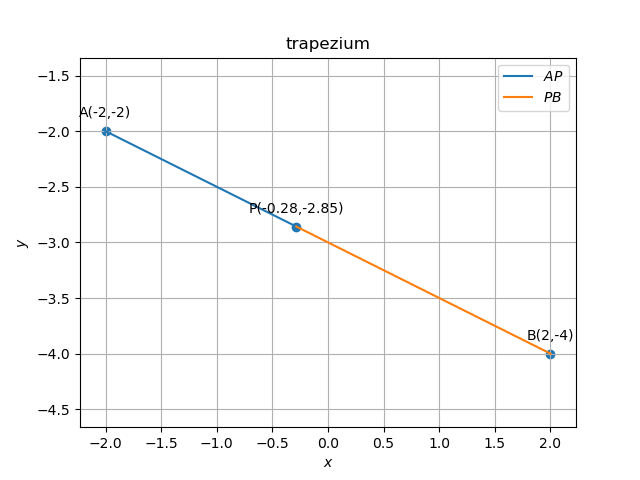
\includegraphics[width=\columnwidth]{chapters/10/7/2/8/figs/vec.png}
   \caption{}
   \label{fig:chapters/10/7/2/8/vec.png}
   \end{figure}
